\section{A declared transport and receiving connection}\label{sec:transport}
The preceding obstruction concerns a particular temporal feedback ansatz. We now introduce a different model with its own state. The inherited delays remain fixed data, while a product measure, two traveling fields, a receiving metric and boundary laws are explicit new choices. Their mathematical feasibility does not select a unique physical realization.

\subsection{Spatial duplication and mixing}
Let $\Lambda=S_L\times G$, $d\mu=ds\,d\ell_X$, and $V=L^2(\Lambda;\R^2)$. Use the same U and Y as in~\eqref{eq:spaces}. Define
\begin{align}
(JQ)(s,X)&=\frac{Q(s)}{\sqrt M},&
(J^*v)(s)&=\frac1{\sqrt M}\int_Gv(s,X)\dd\ell_X,\label{eq:J}\\
(Cv)(X)&=a_o\sqrt M\int_{S_L}\frac{A_sv(s,X)}{d_X(s)}\dd s,&
(C^*\zeta)(s,X)&=\frac{a_o\sqrt M}{d_X(s)}A_s^*\zeta(X).\label{eq:Cspatial}
\end{align}
\begin{proposition}[Exact spatial factorization]\label{prop:factorization}
J is an isometry, $J^*J=I_U$, and $\norm C=\norm{C^*}\le a_o\sqrt{LM}/\delta_w$. With $(D_\theta h)(s,X,t)=h(s,X,t-\theta_X(s))$ on supplied histories,
\begin{equation}\label{eq:factorization}
\KG=CD_\theta J.
\end{equation}
The Gram operator is pointwise multiplication by a bounded nonnegative matrix:
\begin{equation}\label{eq:Gram}
(CC^*\zeta)(X)=\Gmat(X)\zeta(X),\qquad
\Gmat(X)=a_o^2M\int_{S_L}\frac{\operatorname{diag}(1,\hat t(s)\hat t(s)^T)}{d_X(s)^2}\dd s.
\end{equation}
Its scalar block $m_0(X)$ is strictly positive, whereas its vector block may have a kernel.
\end{proposition}
\begin{proof}
Integration over G gives $\norm{JQ}_V^2=M^{-1}M\norm Q_U^2$. Fubini proves both adjoint formulas. Cauchy--Schwarz in s gives
$\norm{Cv}_Y^2\le a_o^2ML\delta_w^{-2}\norm v_V^2$.
The $\sqrt M$ factors cancel in $CD_\theta J$, proving~\eqref{eq:factorization}; time translation/Fubini give its a.e. history interpretation as in Theorem~\ref{thm:observation}. Since $A_sA_s^*=\operatorname{diag}(1,\hat t\hat t^T)$, composition gives~\eqref{eq:Gram}. Its quadratic form is an integral of
$a_o^2Md^{-2}(|\zeta_{\rm sc}|^2+|\hat t\cdot\zeta_v|^2)$, so it is nonnegative and bounded by $a_o^2ML\delta_w^{-2}|\zeta|^2$. In particular
\begin{equation}\label{eq:scalarGram}
0<\frac{a_o^2ML}{(c_e\theta_+)^2}\le
m_0(X)=a_o^2M\int_{S_L}d_X(s)^{-2}\dd s
\le\frac{a_o^2ML}{\delta_w^2}.
\end{equation}
If n is normal to the selected carrier plane, $\hat t(s)\cdot n=0$. Hence $(0,h(X)n)\in\ker C^*$ for any $h\in L^2(G)$; no inverse of $CC^*$ is available in general.
\end{proof}

C and $C^*$ are same-time spatial maps. The construction makes no assumption $\norm C\le1$: cancellation will use conjugate effort/flow pairings, not a claim that C is a unit-power scattering transfer. J is unrelated to the native derivative $J_f$, and $\Gmat$ is unrelated to the old profile operator $\Bcal$.

\subsection{Two traveling states and their time traces}
For each label $(s,X)$ introduce an internal time/age $0<\xi<\theta_X(s)$. Let
\begin{equation}\label{eq:lineSpace}
\Dcal=\{(s,X,\xi):0<\xi<\theta_X(s)\},\qquad
\Wcal=L^2(\Dcal;\R^2)\oplus L^2(\Dcal;\R^2).
\end{equation}
The proposed state laws and oriented boundary signals are
\begin{equation}\label{eq:transportPDE}
\partial_tu_++\partial_\xi u_+=0,\qquad
\partial_tu_--\partial_\xi u_-=0,
\qquad a=u_+(0),\ b=u_-(0),\ c=u_+(\theta),\ d=u_-(\theta).
\end{equation}
Thus a and d are inflows; c and b are outflows. These senses are directions in an abstract channel, not the upper/lower G labels or a toroidal path.

\begin{lemma}[Characteristics, traces and transport work]\label{lem:transport}
For arbitrary $u_{+,0},u_{-,0}$ of finite energy and locally L2 time inflows a,d, the characteristic solution is, a.e.,
\begin{align}
u_+(s,X,\xi,t)&=\begin{cases}
u_{+,0}(s,X,\xi-t),&t<\xi,\\a(s,X,t-\xi),&t\ge\xi,
\end{cases}\label{eq:charplus}\\
u_-(s,X,\xi,t)&=\begin{cases}
u_{-,0}(s,X,\xi+t),&t<\theta_X(s)-\xi,\\
d(s,X,t-\theta_X(s)+\xi),&t\ge\theta_X(s)-\xi.
\end{cases}\label{eq:charminus}
\end{align}
It is continuous in $\Wcal$, and its outflows are legitimate locally L2 time traces:
\begin{align}
c&=\ii_{0\le t<\theta}u_{+,0}(s,X,\theta-t)+\ii_{t\ge\theta}a(s,X,t-\theta),\label{eq:cstartup}\\
b&=\ii_{0\le t<\theta}u_{-,0}(s,X,t)+\ii_{t\ge\theta}d(s,X,t-\theta).\label{eq:bstartup}
\end{align}
Here and below $\theta=\theta_X(s)$ within a channel. With
\begin{align}
E_{\rm tr}(t)&=\frac12\int_\Lambda\int_0^\theta(|u_+|^2+|u_-|^2)\dd\xi\dd\mu\ge0,\label{eq:Etr}\\
P_N&=\tfrac12(\norm a_V^2-\norm b_V^2),&
P_G&=\tfrac12(\norm c_V^2-\norm d_V^2),\label{eq:portpowers}
\end{align}
the exact finite-time account is
\begin{equation}\label{eq:linebalance}
E_{\rm tr}(T)-E_{\rm tr}(0)=\int_0^T(P_N-P_G)\dd t.
\end{equation}
\end{lemma}
\begin{proof}
Following the forward characteristic to time zero or the near inflow gives~\eqref{eq:charplus}. For the backward field, reflect the fixed fiber by $\eta=\theta-\xi$. This is an isometry in fiber L2 and converts the equation to forward transport with inflow d, giving~\eqref{eq:charminus} and both outflows.

For any H, time substitution and Fubini yield
\begin{align}
\int_0^H\norm{c(t)}_V^2\dd t&\le\norm{u_{+,0}}_{L^2(\Dcal)}^2+\int_0^H\norm{a(t)}_V^2\dd t,\notag\\
\int_0^H\norm{b(t)}_V^2\dd t&\le\norm{u_{-,0}}_{L^2(\Dcal)}^2+\int_0^H\norm{d(t)}_V^2\dd t.\label{eq:tracebounds}
\end{align}
Startup and delayed terms occupy disjoint time intervals for each channel, so there is no extra factor two. The startup substitutions are $\xi=\theta-t$ and $\xi=t$; delayed terms translate time with unit Jacobian. These bounds applied to null differences prove representative independence in $(s,X,t)$. They do not give prescribed instantaneous boundary values of general L2 profiles.

For continuity, extend a forward initial profile by zero to the whole real $\xi$ line, and extend the inflow by zero to negative time and beyond a fixed finite horizon. The characteristic state is the restriction to $\Dcal$ of a translated initial extension plus a reflected, translated inflow extension, with disjoint supports except at the null seam. Translation is strongly continuous on $L^2(\Lambda\times\R)$, first on dense smooth finite sums and then by isometry. Restriction is bounded. This proves continuity including time zero; the fixed fiber reflection proves the same for $u_-$. No corner matching is needed.

For a fixed forward channel with delay $\theta$, initial profile $v_0$ and inflow h, direct substitution gives
\begin{equation}\label{eq:fiberenergy}
\int_0^\theta|v(\xi,t)|^2\dd\xi
=\int_0^{(\theta-t)_+}|v_0(\eta)|^2\dd\eta
+\int_{(t-\theta)_+}^{t}|h(r)|^2\dd r.
\end{equation}
Subtract the initial norm. The lost initial portion is the time integral of startup outflow; the input already exited is its delayed outflow. Thus the change equals $\int_0^t(|h|^2-|o|^2)\dd r$. Integrate over labels and apply this to both orientations, using~\eqref{eq:tracebounds} for integrability. Half the sum is exactly~\eqref{eq:linebalance}. The energy is absolutely continuous, with the derivative identity a.e., and the continuous state determines its endpoint values.
\end{proof}

This is an energy-space proof, not integration by parts at nonexistent Sobolev traces. Static delays contribute no time derivative or spatial Jacobian. Unit propagation speed in $\xi$ merely defines the channel time coordinate.

\subsection{Closed coupling and proposed storage metrics}
Choose $\kappa\ge0$, $\beta_G>0$ and a new field $\zeta\in Y$. Retain the original x,z equations exactly and declare
\begin{equation}\label{eq:closedmodel}
\boxed{\begin{aligned}
\dot Q&=A_cQ+(\Bcal q,0)+\FF,\\
\FF&=-\kappa^2J^*JQ+\sqrt2\kappa J^*b=-\kappa^2Q+\sqrt2\kappa J^*b,\\
a&=\sqrt2\kappa JQ-b,\\
d&=\sqrt2C^*\zeta-c,\\
\beta_G\dot\zeta&=\sqrt2Cc-CC^*\zeta.
\end{aligned}}
\end{equation}
Together with~\eqref{eq:transportPDE}, the characteristic inflows/outflows and the retained finite-dimensional equations, this specifies the whole exchange-stage model. Its near effort/flow variables are
\begin{equation}\label{eq:effortflow}
e_N=\frac{a+b}{\sqrt2}=\kappa JQ,\quad f_N=\frac{a-b}{\sqrt2},\qquad
e_G=\frac{c+d}{\sqrt2}=C^*\zeta,\quad f_G=\frac{c-d}{\sqrt2}.
\end{equation}
Solving these relations with $\FF=-\kappa J^*f_N$ and $\beta_G\dot\zeta=Cf_G$ gives every sign and $\sqrt2$ factor in~\eqref{eq:closedmodel}. Define
\begin{equation}\label{eq:augmentedstocks}
H_G=\frac{\beta_G}{2}\norm\zeta_Y^2,\qquad H_{\rm total}=H_{\rm RX}+E_{\rm tr}+H_G.
\end{equation}
The new field does not relocate old z; old $H_R$ is counted once inside $H_{\rm RX}$.

The Hilbert identity $\langle(v+w)/\sqrt2,(v-w)/\sqrt2\rangle=(\norm v^2-\norm w^2)/2$ gives the component algebra
\begin{equation}\label{eq:componentpowers}
\ip{Q}{\FF}_U=-P_N,
\qquad \ip{\zeta}{\sqrt2Cc-CC^*\zeta}_Y=P_G.
\end{equation}
Equivalently these powers are $-\kappa^2\norm Q^2+\sqrt2\kappa\langle JQ,b\rangle$ and $\sqrt2\langle C^*\zeta,c\rangle-\norm{C^*\zeta}^2$. Their regularity justification for the mild model comes next. Apparent damping transfers energy to modeled traveling states rather than to an omitted sink.

\begin{figure}[htbp]\centering
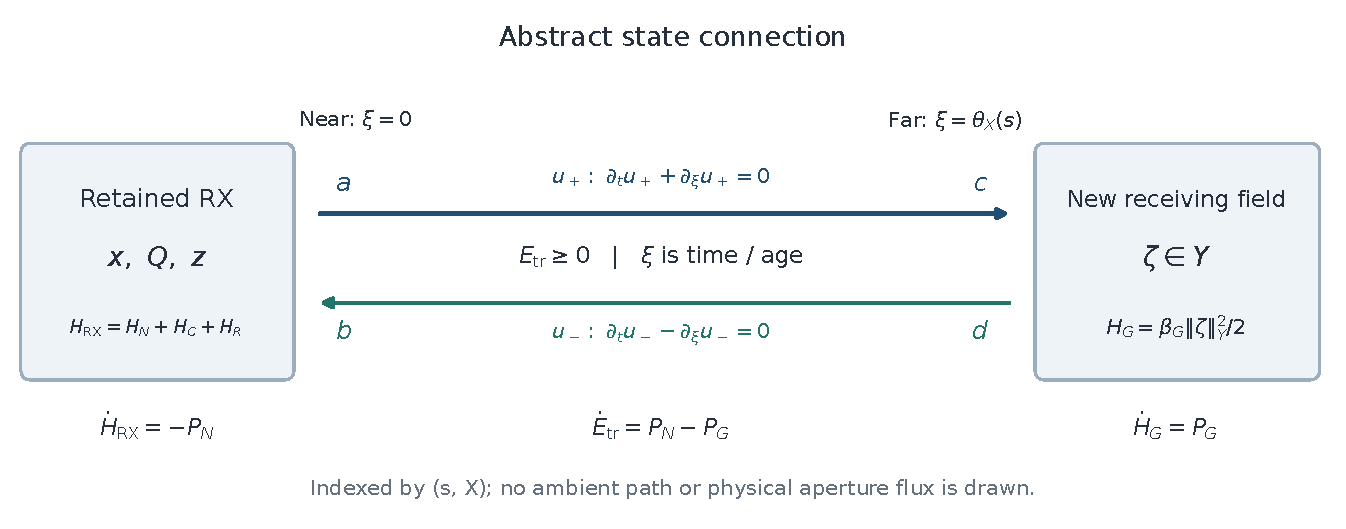
\includegraphics[width=\textwidth]{figures/channel_account.pdf}
\caption{Abstract state connection for a representative channel label $(s,X)$. The near and far powers are sums over the product measure, not physical aperture fluxes. C mixes carrier labels at each X; the receiving field is not six independent point receivers. The coordinate $\xi$ is time/age, and the diagram specifies no ambient curved route.}\label{fig:channel}
\end{figure}
